\chapter{Ionosphere Incoherent Scatter Spectrum}
\label{appendix1}
\thispagestyle{myheadings}
\graphicspath{{Appendix/Figures/}}

%%%%%%%%%%%%%%%%%%%%%%%%%%%%%%%%%%%%%%%%%%%%%%%%%%%%%%%%%%%%%%%%%%%%%%%%%

This is the mathematical basis for calculating incoherent scatter spectrum for a given set of ionosphere state parameters. The appendix uses the methods developed \cite{kudeki:milla:1} and \cite{Kudeki:2006kx}.

\section*{Overall Formulation}
The first step comes from \cite{kudeki:milla:1} where a lumped circuit model is used to describe the spectrum. In it the independent thermal fluctuations of each species of ions and electrons are treated as current sources and the macroscopic conductances are treated as discrete components. The electric field $E$ impinged from the radar acts as a voltage. This lumped circuit model, seen in Figure \ref{fig:circuit}, is derived is taking the scalar component of Ampere's law in the direction of $\mathbf{k}$.  

\begin{equation}
\label{eq:ampere}
-j\mathbf{k} \times \mathbf{H} = \mathbf{J} +j\omega \epsilon_0 \mathbf{E},
\end{equation}

\noindent which then yields,

\begin{equation} 
\label{eq:ampscaler}
0=(\sigma_i +\sigma_e)E +\frac{\omega}{k}e(n_{ti}-n_{te}) +j\omega \epsilon_0 E.
\end{equation}

\begin{figure}[!h]
\centering
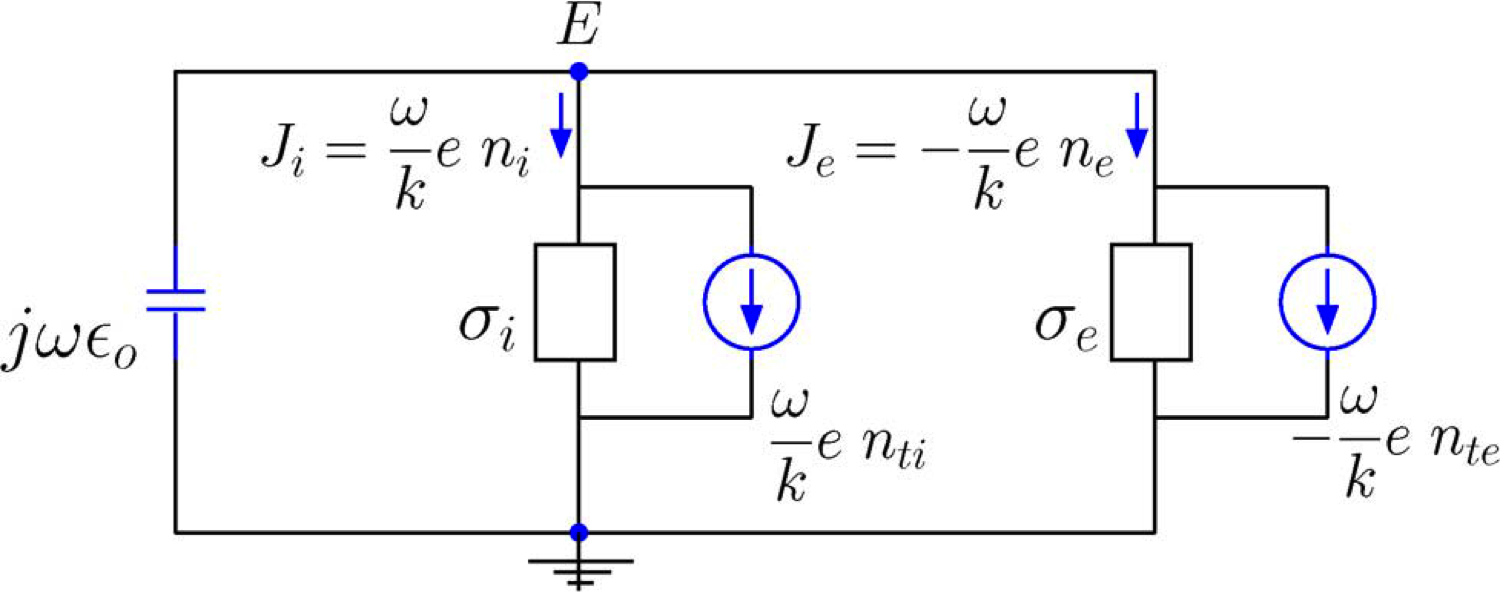
\includegraphics[width=3.0in]{circuit}
% where an .eps filename suffix will be assumed under latex, 
% and a .pdf suffix will be assumed for pdflatex; or what has been declared
% via \DeclareGraphicsExtensions.
\caption{Lumped circuit model seen in  \cite{kudeki:milla:1}.}
\label{fig:circuit}
\end{figure}

\noindent Using the electron current expression, $-\omega k^{-1}en_e = E\sigma_e -\omega k^{-1}en_{te}$, these equations can be rearranged to solve for $n_e$, 

\begin{equation}
\label{eq:neeq}
n_e(\mathbf{k},\omega) =  \frac{(j\omega\epsilon_0 + \sigma_i) n_{te}(\mathbf{k},\omega)}{j\omega\epsilon_0 +\sigma_e+\sigma_i} + \frac{\sigma_en_{ti}(\mathbf{k},\omega)}{j\omega\epsilon_0 +\sigma_e+\sigma_i}.
\end{equation}

\noindent To determine the power spectrum we square and average Equation \ref{eq:neeq} taking into account that the terms $n_{te}$ and $n_{ti}$ are independent of one and other we result in the following
\begin{equation}
\label{mainspeceq}
\langle \left|n_e(\mathbf{k},\omega)\right|^2\rangle = \frac{|j\omega\epsilon_0 + \sigma_i|^2 \langle |n_{te}(\mathbf{k},\omega)|^2\rangle}{|j\omega\epsilon_0 +\sigma_e+\sigma_i|^2} + \frac{| \sigma_e|^2 \langle |n_{ti}(\mathbf{k},\omega)|^2\rangle}{|j\omega\epsilon_0 +\sigma_e+\sigma_i|^2}.
\end{equation}

We can generalize them for multiple ion species by simply summing over the thermal fluctuations and conductances in Equation \ref{eq:ampscaler},

\begin{equation} 
\label{eq:ampscalersum}
0=\left(\displaystyle \sum_k^K\sigma_{ik} +\sigma_e\right)E +\frac{\omega}{k}e\left(\sum_k^Kn_{tik}-n_{te}\right) +j\omega \epsilon_0 E.
\end{equation}

\noindent This then augments the power spectrum in Equation \ref{mainspeceq} to the following

\begin{equation}
\label{eq:sumspeceq}
\displaystyle \langle \left|n_e(\mathbf{k},\omega)\right|^2\rangle = \frac{\left|j\omega\epsilon_0 +  \sum_k^K\sigma_{ik} \right|^2 \langle |n_{te}(\mathbf{k},\omega)|^2\rangle}{\left|j\omega\epsilon_0 +\sigma_e+ \sum_k^K\sigma_{ik} \right|^2} + \frac{| \sigma_e|^2 \left \langle \left|\sum_k^Kn_{tik}(\mathbf{k},\omega)\right|^2\right\rangle}{\left|j\omega\epsilon_0 +\sigma_e+ \sum_k^K\sigma_{ik} \right|^2}.
\end{equation}

%%%%%%%%%%%%%%%%%%%%%%%%%%%%%%%%%%%%%%%%%%%%%%%%%%%%%%%%%%%%%%%%%%%%%%
\section*{Gordeyeve Integrals}
The power spectrum of the thermal fluctuation for each species $s$ can be determined by the following,

\begin{equation}
\label{eq:thermalfl}
\frac{\langle|n_{ts}(\mathbf{k},\omega)|^2\rangle}{N_s} = 2\text{Re}\{J_s(\omega_s)\},
\end{equation}

\noindent where $N_s$ is the average density for the species.  Also the conductance for each species $s$ can be determine from the following,

\begin{equation}
\label{eq:cond}
\frac{\sigma_{s}(\mathbf{k},\omega)}{j\omega\epsilon_0} = \frac{1-j\omega_s J_s(\omega_s)}{k^2\lambda_s^2}
\end{equation}

\noindent where $\omega_s \equiv \omega-\mathbf{k}\cdot\mathbf{V}_s $ is the Doppler shifted frequency and $\lambda_s \equiv \sqrt{\frac{\epsilon_0 KT_s}{N_s q_s^2}}$ is the Debye length for each species.

The $J_s$ terms can be represented as follows

\begin{equation}
\label{eq:gord}
J_s(\omega)\equiv \int_0^\infty \langle e^{j\mathbf{k}\cdot\Delta \mathbf{r}_s}\rangle e^{j\omega\tau}d\tau
\end{equation}

\noindent These terms are known as Gordeyeve integrals, which are the one sided Fourier transforms of the characteristic functions of the particle displacements $\langle e^{j\mathbf{k}\cdot\Delta\mathbf{r}_s}\rangle$.  

The particle displacement function can change depending on magnetic field and collisionality of the plasma. For the high latitude F-region in the ionosphere a case of general importance is one of a non-magnitized and collision less plasma, where $\Delta\mathbf{r} = \mathbf{v}\tau$ where $\tau$ is the time interval. Assuming a Maxwellian the PDF of one dimensional displacement is

\begin{equation}
\label{eq:pdfr}
f(\Delta r) = \frac{1}{\sqrt{2\pi \langle r^2 \rangle}}e^{\frac{-\Delta r^2}{2\langle r^2\rangle}}.
\end{equation}
 
\noindent The variance term $\langle r^2 \rangle$ can be represented as
\begin{equation}
\label{eq:var}
\langle r^2 \rangle = \langle v^2 \rangle \tau^2 = \frac{KT_s}{m_s} \tau^2
\end{equation}
 \noindent where $T_s$ is the temperature of the species, $K$ is Boltzmans constant and $m_s$ is the mass of the species in kg. To simplify notation like in \cite{kudeki:milla:1}, we will refer to $\sqrt{KT_s/m_s}$ as $C$. Which yields the following single particle ACF,
 
 \begin{equation}
\label{eq:pdfall}
\langle e^{j\mathbf{k}\cdot\Delta \mathbf{r}}\rangle= e^{-\frac{1}{2}k^2C^2 \tau^2}.
\end{equation}
 
 To model collisions we use the term $\nu$ as the collision frequency for the species. If $\nu<<kC$ then \ref{eq:pdfall} can be used as the single particle ACF. If not the following must be used.
 
 \begin{equation}
 \label{eq:colspacf}
 \langle e^{j\mathbf{k}\cdot\Delta \mathbf{r}}\rangle = e^{-\frac{k^2C^2}{\nu^2}\left( \nu \tau-1+e^{-\nu\tau}\right)}
 \end{equation}
 
Lastly if one is to add a magnetic field to the equations the single particle ACFs must now take into a account the orientation of the magnetic field. The authors of \cite{kudeki:milla:1} use the convention of breaking up the Bragg vector $\mathbf{k}$ into two components, one parallel to the magnetic field, $k_{\parallel}$ and one perpendicular,$k_{\perp}$, as such, $\mathbf{k}= \hat{b}k_{\parallel}+\hat{p}k_{\perp}$. This yields the following formulation for the single particle ACF,

 \begin{equation}
\label{eq:pdfmag}
\langle e^{j\mathbf{k}\cdot\Delta \mathbf{r}}\rangle= e^{-\frac{1}{2}k_{\parallel}^2C^2 \tau^2}\times e^{-\frac{2k_{\perp}^2C^2}{\Omega^2} \sin^2(\Omega\tau/2)},
\end{equation}

\noindent where the gyro frequency is $\Omega = qB/m$This formulation neglects the effects of collisions which if taken into account yields the following single particle ACF,

\begin{equation}
\label{eq:colspacf}
\langle e^{j\mathbf{k}\cdot\Delta \mathbf{r}}\rangle = e^{-\frac{k_\parallel^2C^2}{\nu^2}\left( \nu \tau-1+e^{-\nu\tau}\right)}\times e^{-\frac{k_\perp^2C^2}{\nu^2+\Omega^2}\left(\cos(2\gamma) + \nu \tau-e^{-\nu\tau}\cos(\Omega\tau-2\gamma)\right)},
\end{equation}
 
\noindent where $\gamma = \tan^{-1}(\nu\Omega)$. The for the case with the magnetic field as one gets closer to being fulling perpendicular to $\mathbf{B}$ the single particle ACFs become much more narrow band, to the point of becoming delta functions in the frequency space. It is necessary to use other methods beyond numerical integration to determine the Gordeyeve Integrals. The authors of \cite{kudeki:milla:2} get around this problem by making a PIC code to determine the particle statistics. 


%%%%%%%%%%%%%%%%%%%%%%%%%%%%%%%%%%%%%%%%%%%%%%%%%%%%%%%%%%%%%%%%%%%%%%
 \section*{Computational Considerations}
One of the main challenges to calculating the ISR spectrums is calculating the Gordeyeve integrals. The case with no collisions or magnetic fields can be done analytically using Dawsons integral. This can be done using the identity

\begin{equation}
\label{eq:daw1}
jZ(\theta) = \int_0^{\infty} e^{-j\theta t}e^{-\frac{t^2}{4}}dt = \sqrt{\pi}e^{-\theta^2}-j2e^{-\theta^2}\int_0^\theta e^{t^2}dt.
\end{equation}

\noindent Using the terms found in Equation \ref{eq:pdfall}, $\theta=\omega_s/\left(\sqrt{2}kC\right)$ and $t=\sqrt{2}kC\tau$.

For other cases where analytical calculation is not possible a numerical integration scheme from \cite{Ooi:2007jx} is used. It is also possible to use a Chirp-z based algorithm that is shown in \cite{Li:1991gr} from the experiences of the author the first technique converges faster. The technique used in \cite{Ooi:2007jx} changes the variable of integration for integrals of the following form,

\begin{equation}
\label{eq:Sommer}
I=\int_a^b f(z) dz.
\end{equation}

\noindent The technique changes the variable $z$ in the following way,

\begin{equation}
\label{eq:newz}
z = \frac{1}{2}(a+b)+\frac{1}{2} (b-a)\text{Erf}(g(t)),
\end{equation}

\noindent where $g(t)$ is a function that is choosen so  $g(t)\rightarrow\pm \infty$ as $t\rightarrow\pm \infty$ and $Erf(u)$ is 
\begin{equation}
\label{eq:erf1}
\text{Erf}(u) = \frac{2}{\sqrt{\pi}}\int_0^u e^{-t^2}dt.
\end{equation}

\noindent Discretizing and changing variables the integral in Equation \ref{eq:Sommer} becomes the following sum

\begin{equation}
\label{eq:erfsum1}
I=\displaystyle \sum_{n=-N}^N A_nf\left( \frac{1}{2}(a+b)+\frac{1}{2} (b-a)\text{Erf}(g(nh))\right)
\end{equation}

\noindent where,
\begin{equation}
\label{eq:anterm}
A_n = g'(nh)e^{-g(nh)^2}.
\end{equation}

\noindent Like in \cite{Ooi:2007jx}, $g(nh) = \sinh (nh)$ and the grid spacing $h$ is the following,

\begin{equation}
\label{eq:hterm}
h = \frac{1}{N}\ln(1.05\sqrt{2}N).
\end{equation} 


Lastly to avoid cases of divid by zero errors the main equations have to be rearrange slightly. First off because some ion species could have zero density Equation \ref{eq:cond} uses the Debye length of the electron species,$\lambda_e$ as follows

\begin{equation}
\label{eq:condnew}
\frac{\sigma_{s}(\mathbf{k},\omega)}{j\omega\epsilon_0} = \frac{1-j\omega_s J_s(\omega_s)}{k^2\lambda_e^2} \left(\frac{q_sT_eN_s}{q_eT_sN_e}\right).
\end{equation}

Also, to avoid having to more calculations then necessary the $j\omega\epsilon_0$. terms of Equation \ref{eq:sumspeceq} are moved around. Thus it becomes,

\begin{equation}
\label{eq:sumspeceqfinal}
\displaystyle \langle \left|n_e(\mathbf{k},\omega)\right|^2\rangle =  \frac{\left|1 +  \sum_k^K\frac{\sigma_{ik}}{j\omega\epsilon_0} \right|^2 \langle |n_{te}(\mathbf{k},\omega)|^2\rangle}{\left|1 +\frac{\sigma_e+ \sum_k^K\sigma_{ik}}{j\omega\epsilon_0} \right|^2} + \frac{\left| \frac{\sigma_e}{j\omega\epsilon_0} \right|^2\left \langle \left|\sum_k^Kn_{tik}(\mathbf{k},\omega)\right|^2\right\rangle}{\left|1 +\frac{\sigma_e+ \sum_k^K\sigma_{ik}}{j\omega\epsilon_0} \right|^2}.
\end{equation}

\noindent If the Gordeyeve integrals are substitute in Equation \ref{eq:sumspeceqfinal} it becomes the following.

\begin{equation}
\label{eq:sumspeceqactual}
\displaystyle \langle \left|n_e(\mathbf{k},\omega)\right|^2\rangle =  \frac{\left|1 + \sum_s^K  \frac{1-j\omega_s J_s(\omega_s)}{k^2\lambda_e^2} \left(\frac{q_sT_eN_s}{q_eT_sN_e}\right) \right|^2 2N_e\text{Re}\{J_e(\omega_e)\}}{\left|1 + \frac{1-j\omega_e J_e(\omega_e)}{k^2\lambda_e^2}  +\sum_s^K  \frac{1-j\omega_s J_s(\omega_s)}{k^2\lambda_e^2} \left(\frac{q_sT_eN_s}{q_eT_sN_e}\right) \right|^2}       +                 \frac{\left| \frac{1-j\omega_s J_e(\omega_e)}{k^2\lambda_e^2} \right|^2\sum_s^K  2N_s\text{Re}\{J_s(\omega_s)\}}{\left|1 + \frac{1-j\omega_e J_e(\omega_e)}{k^2\lambda_e^2}  +\sum_s^K  \frac{1-j\omega_s J_s(\omega_s)}{k^2\lambda_e^2} \left(\frac{q_sT_eN_s}{q_eT_sN_e}\right) \right|^2}.
\end{equation}

\section*{Examples}
We can see in Figure \ref{fig:diffspectrums} examples of ISR spectrums from different ISR systems. The spectrums were generated using the the parameters values $N_e=1e11$, $T_e=3000^o$K and $T_i=3000^o$K and the system parameter values seen in Table \ref{tab:ISRsys}. The ion acoustic frequency$f_{ia}$ for each system with the following plasma parameters its wavelength $\lambda$ was calculated using the following formula,

\begin{equation}
\label{eq:iaf}
f_{ia} = \frac{\lambda}{2}\sqrt{\frac{k_bT_e +k_b\gamma_iT_i}{M}},
\end{equation}

\noindent where $M$ is the ion mass in kg, $k_b$ is Botlzmann's constant and $\gamma_i$ is the adiabatic index which is set to 3 in all cases. In most of the cases the familiar double hump spectrum is visible. The only exception to this is Jicamarca, where the system's k-vector is very close to being perpendicular to the earths magnetic field. This also impacts the amount of time it takes to calculate the spectrum because as the k-vector gets closer to being perpendicular to magnetic field the Gordeyeve integral will take longer to converge.
\begin{figure}[!h]
\centering
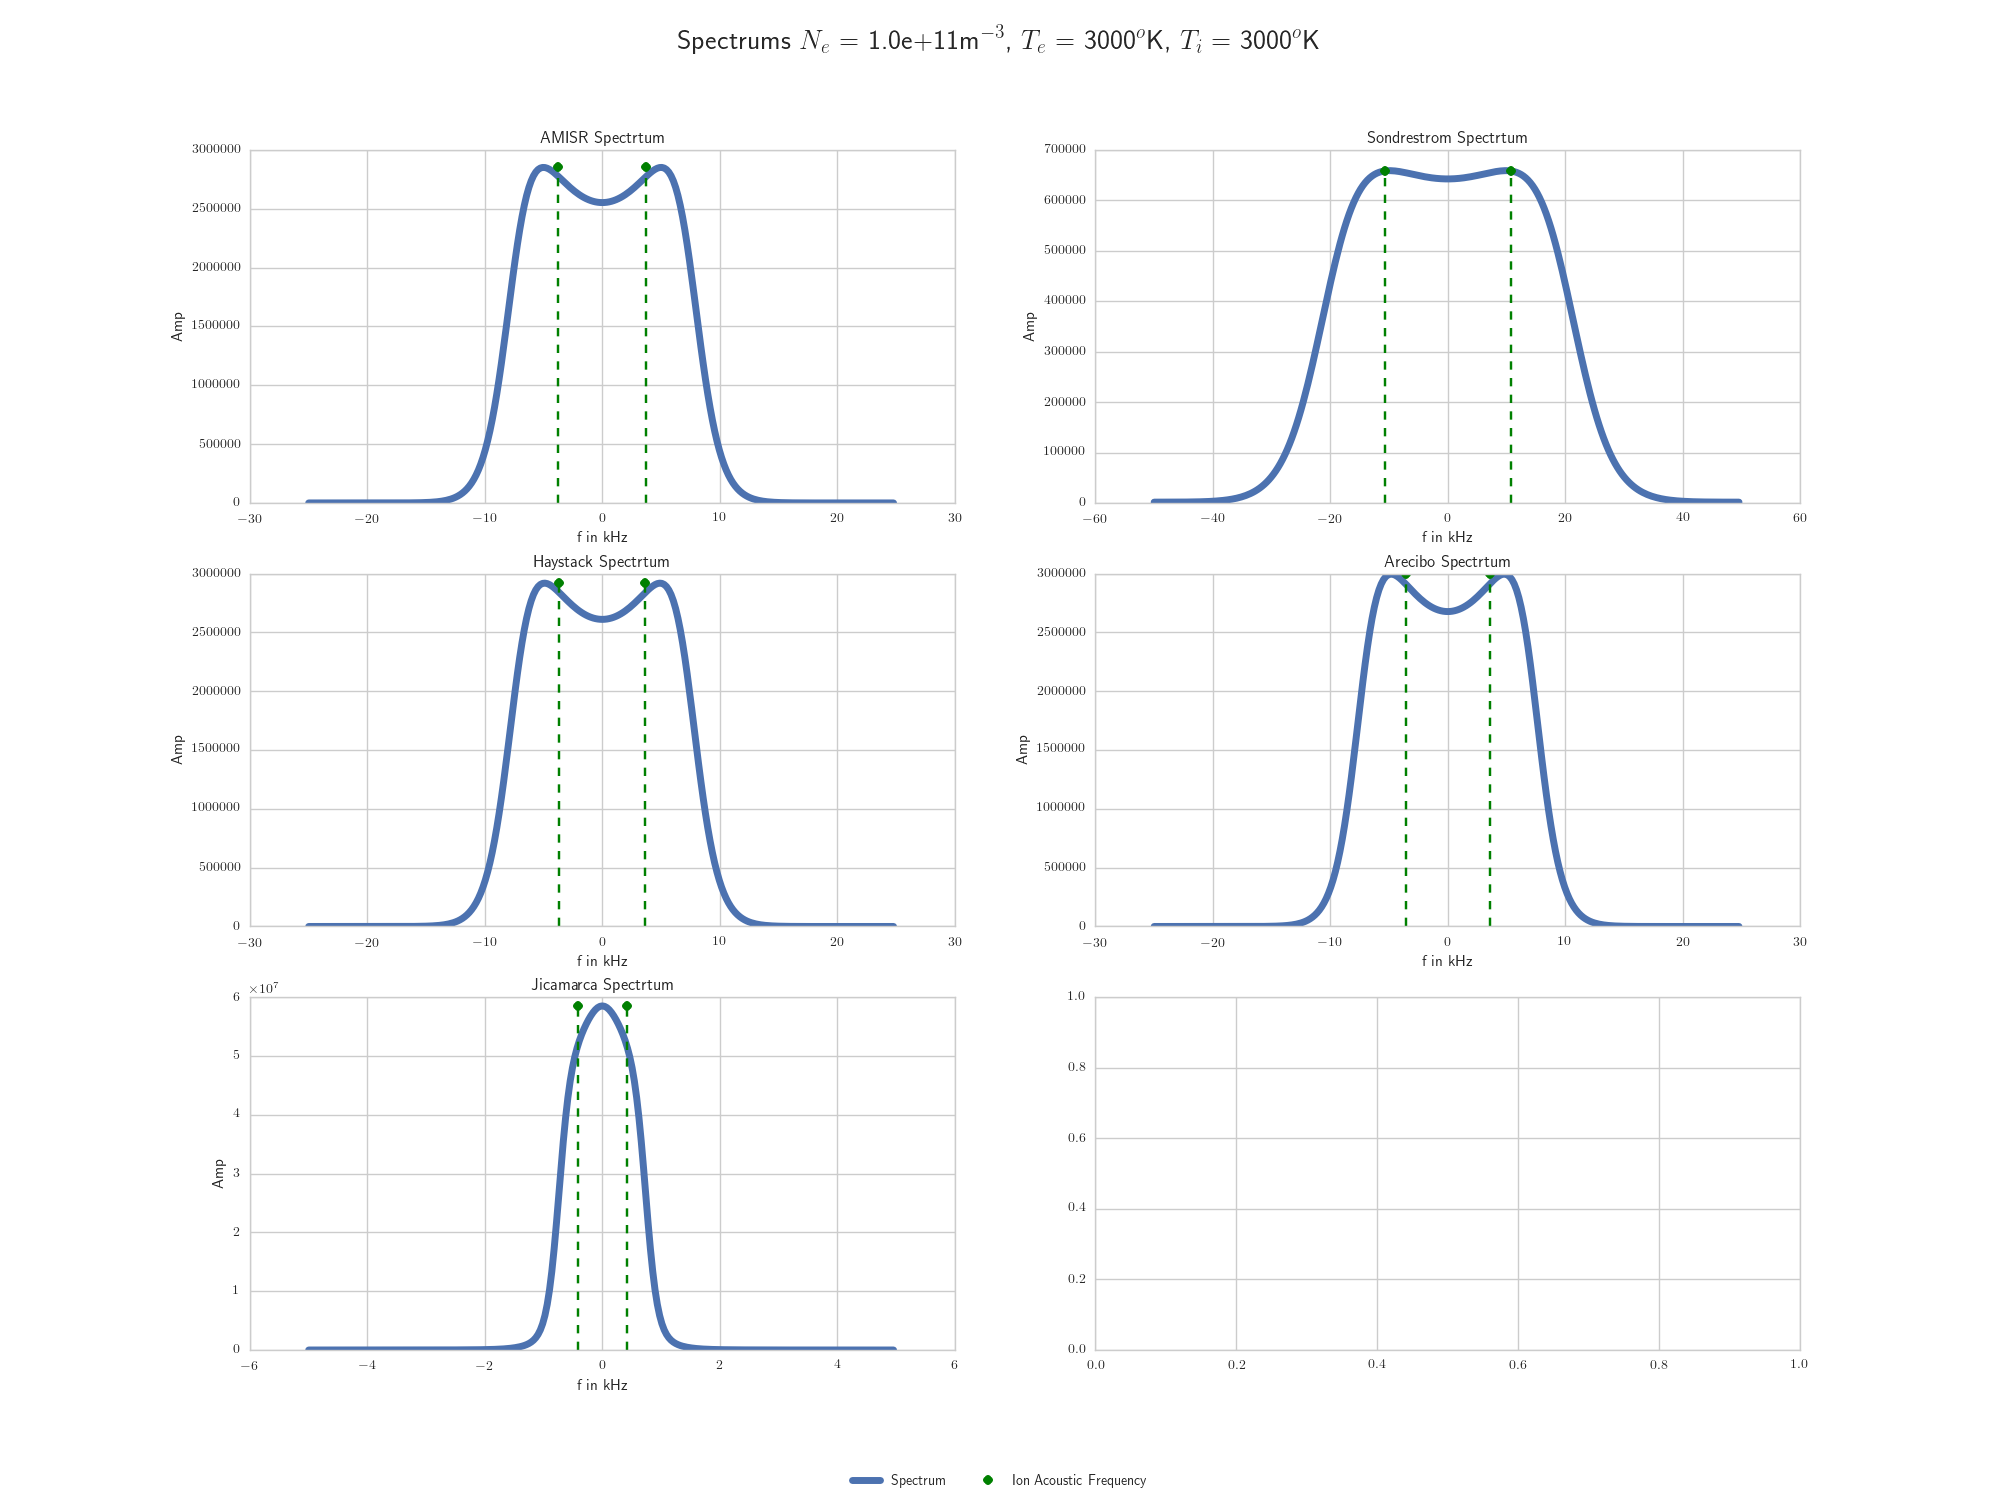
\includegraphics[width=7.0in]{DifferentSystems}

\caption{Spectrums From Different ISR Systems}
\label{fig:diffspectrums}
\end{figure}


\begin{table}[!h]
\centering
\caption{ISR System Parameters}
\label{tab:ISRsys}
\begin{tabular}{lllll}
System Name & $f_0$ in MHz & $f_s$ in kHz & $\alpha$ in $^o$ &  \\
AMISR       & 449          & 50           & 70               &  \\
Sondrestrom & 1290         & 100          & 80               &  \\
Haystack    & 440          & 50           & 65               &  \\
Arecibo     & 430          & 50           & 45               &  \\
Jicamarca   & 50           & 10           & 1                & 
\end{tabular}
\end{table}